\documentclass[paper slide]{beamer}
\usetheme{Boadilla}
\usepackage{essay-def}
\usepackage{bm}
\usepackage{amsfonts}
\usepackage{amssymb}
\usepackage{amsmath}
\usepackage{amsthm}
\usepackage{comment}
\usepackage{subcaption}
\usepackage{geometry}
\usepackage{algorithmic}
\usepackage{algpseudocode}
\usepackage{algorithmicx}
\geometry{left=1cm,right=1cm}
    \title[Probabilistic SGS modeling]{A probabilistic approach to 
		subgrid-scale modeling}
\author[J. Zhao]{Jiaxi Zhao \\ \small joint with Q. Li\@ NUS, N. Thuerey\@ TMU}
\date[\today]{NUS-SJTU PhD Forum \\ \today}
\begin{document}
\par \setlength{\parindent}{2em}

\begin{frame}
\titlepage
\end{frame}


\begin{frame}{Content}
	\begin{itemize}
		\item 1. Difficulties encountered in the data-driven turbulence modeling.
		\item 2. Possible explanation of the problem on 1D Kuramoto–Sivashinsky
		equation.
		\item 3. An effective probabilistic SGS model that improves the
		regression-based method.
	\end{itemize}
\end{frame}


\begin{frame}{Motivation:}
	\begin{itemize}
		\item 1. Performing DNS is unaffordable, even a LES with 50M grids of length 1000s takes several days.
		\item 2. Cheap simulation such as RANS and coarse-grid LES can not obtain accurate quantities such as peak pressure.
	\end{itemize}
	\begin{figure}[ht]
		\centering
		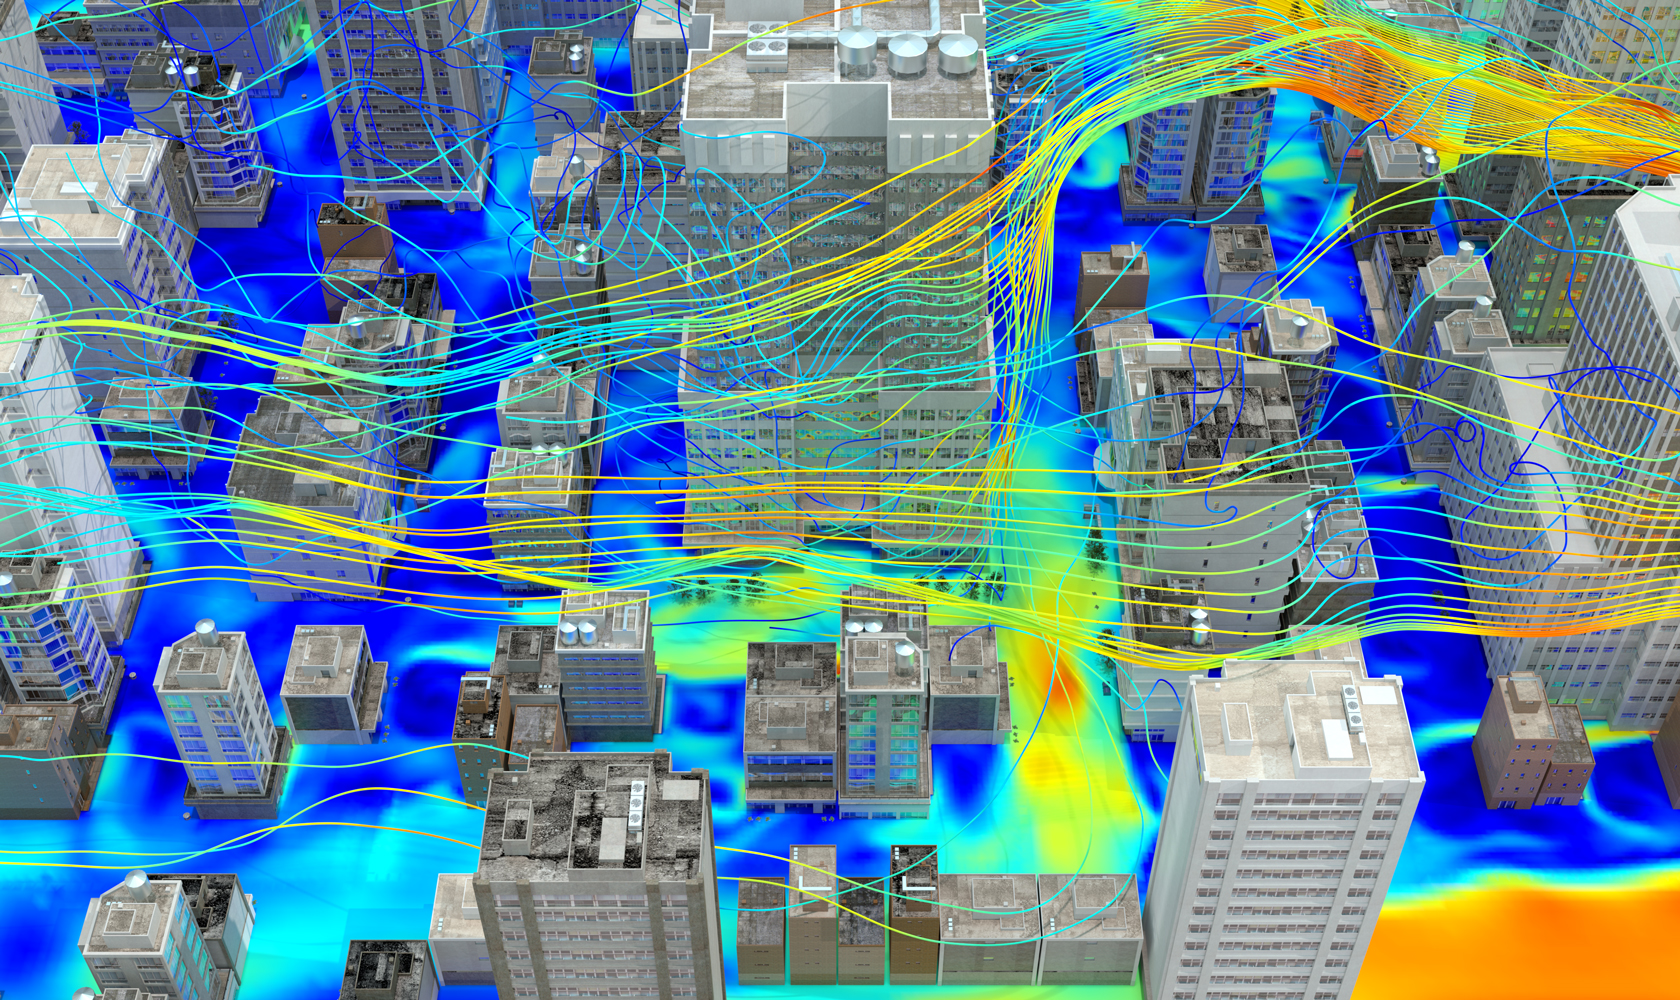
\includegraphics[width=.6\linewidth]{fig/urban_environment.jpeg}
	\end{figure}
	\textit{Can we {\color{red}design or learn better SGS models} based on the LES data so that it can achieve accurate
	results even {\color{red}on coarse grid LES?}}
\end{frame}


\begin{frame}{Subgrid-scale stress modeling based on NN}
	\begin{equation*}
		\begin{aligned}
		\frac{\p u_i}{\p t} + \frac{\p}{\p x_j}(u_iu_j) & \ = 
		-\frac{\p p}{\p x_i} + \nu\Delta u_i,   \\
		\frac{\p u_i}{\p x_i} & \ = 0.
		\end{aligned}
	\end{equation*}
	Applying a filter $G$ to the equation, i.e. 
	$\overline{u} = G * u$
	\begin{equation*}
		\begin{aligned}
		\frac{\p \overline{u}_i}{\p t} + \frac{\p}{\p x_j}(\overline{u}_i
		\overline{u}_j) & \ = -\frac{\p \overline{p}}{\p x_i} + \nu\Delta 
		\overline{u}_i - \frac{\p \tau_{ij}}{\p x_j},   \\
		\frac{\p \overline{u}_i}{\p x_i} & \ = 0,		\\
		\tau_{ij} & \ = \overline{u_iu_j} - \overline{u}_i\overline{u}_j.
		\end{aligned}
	\end{equation*}
	Classical SGS stress models include the (dynamic) Smagorinsky model, 
	and the Wall-Adapting Local Eddy-Viscosity model, and etc. They all based
	on physical intuition and empirical data.
\end{frame}


\begin{frame}{Data-driven SGS stress modeling}
	Machine learning brings powerful approximation toolbox for the development
	of SGS stress models. Most existing works can be summarized to the following
	three categories:
	\begin{itemize}
		\item 1. Rely on classical turbulence models, e.g. Smagorinsky model and
		use DNS data to fit the model parameters.
		\item 2. Choose the input features and fit an end-to-end mapping between
		them and the QoI.
		\item 3. View the SGS stress modeling as a policy and solve it in the
		framework of reinforcement learning.
	\end{itemize}
	Global SGS model is impossible because of the computational cost and data
	sparsity.
\end{frame}


\begin{frame}{SGS stress modeling}
	There are three main issues for stress modeling:
	\begin{itemize}
		\item 1. The mapping from the input features. e.g. filtered velocity to the
		stress tensor is {\color{red}non-deterministic} while
		most classical turbulence models and data-driven models are deterministic.
		\begin{equation*}
			\overline{u}, \nabla \overline{u}, \overline{p} 
			\overset{\text{NOT DETERMINISTIC}}{\Longrightarrow} \tau, \quad 
			\min_{\phi}\norml \tau - \phi(\overline{u}) \normr^2.
		\end{equation*}
		\item 2. Discrepancy between 
		{\color{red}a-priori error and a-posteriori error}.
		\begin{equation*}
			\norml \wht\tau - \tau \normr^2, \quad \norml \overline{u}(T) -
			\overline{u}(T) \normr^2
		\end{equation*}
		This is very different from classical numerical analysis perspective where
		a smaller truncation error (higher order) mostly indicates faster
		convergence via the Lax equivalence theorem.
		\item 3. Difficult to combine the OpenFOAM solver with gradient-based
		optimization algorithms.
	\end{itemize}
\end{frame}


\begin{frame}{A-priori and a-posteriori discrepancy}
	The inconsistency between the a priori error and a posteriori error arises because the {\color{red}training algorithm does not take the solver dynamics into account}.
	\begin{figure}
		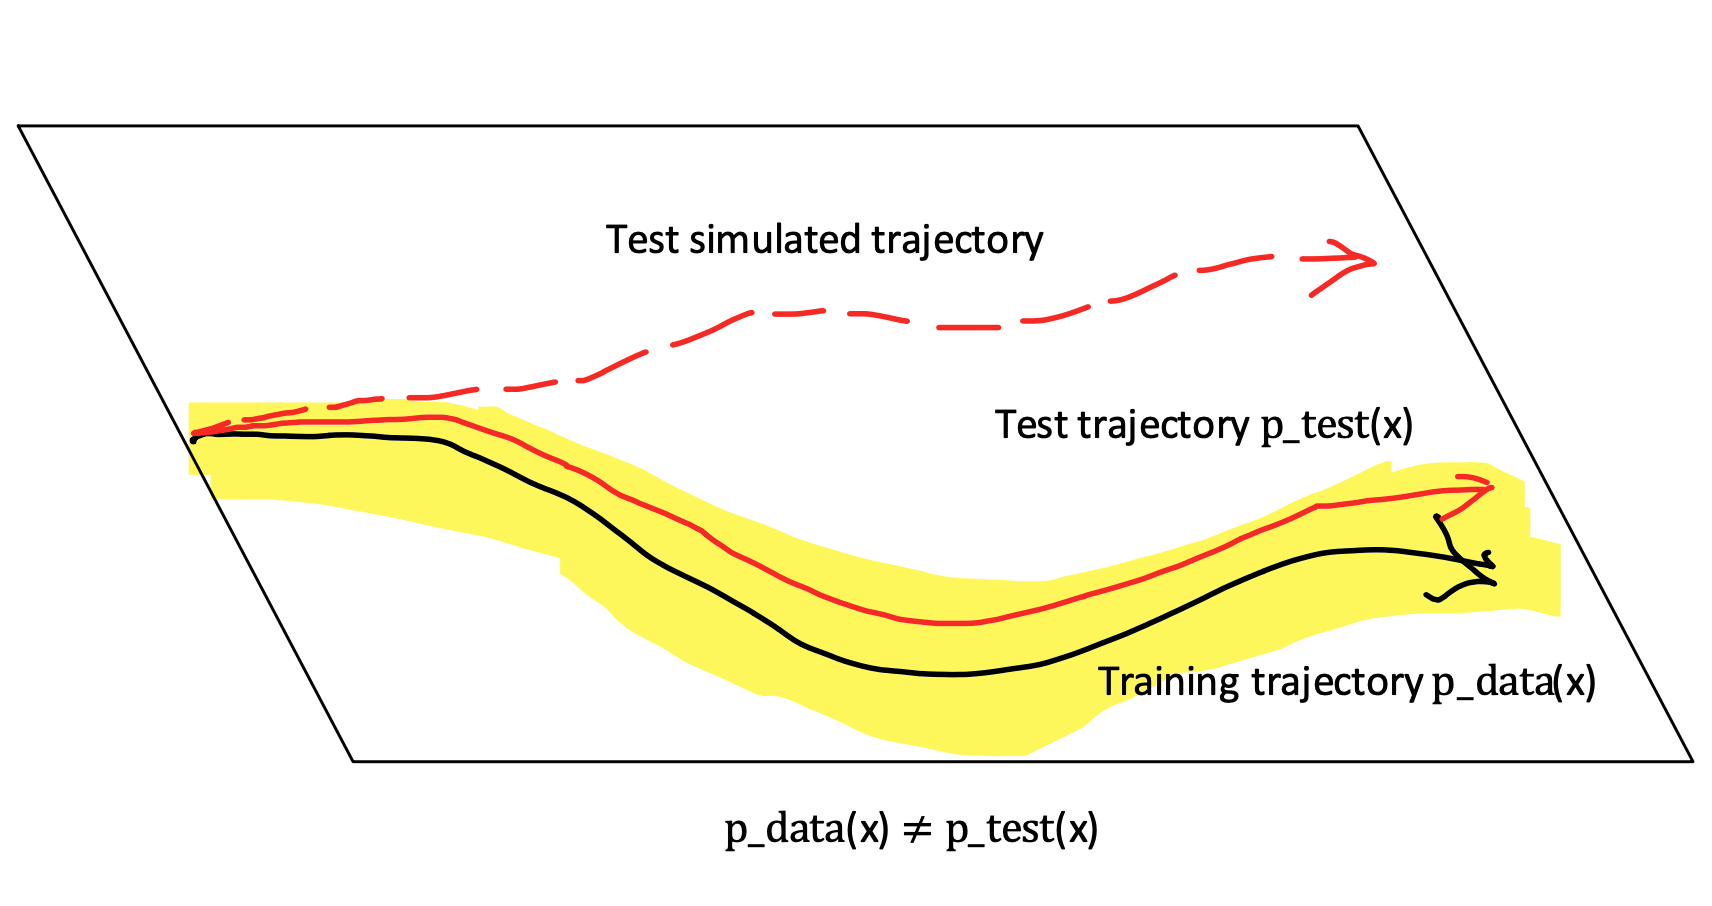
\includegraphics[width=.6\textwidth]{fig/dilemma.png}
		\label{fig:dilemma}
	\end{figure}
	The a-priori and a-posteriori performance are not consistent.
	\begin{figure}
		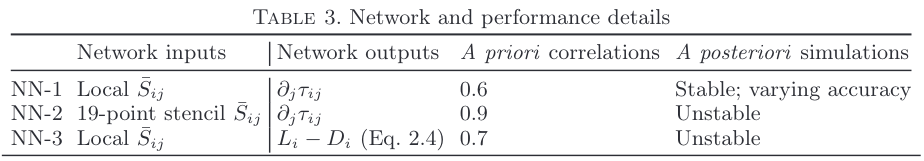
\includegraphics[width=.8\textwidth]{fig/dichotomy.jpg}
		\label{fig:dichotomy}
	\end{figure}
\end{frame}


\begin{frame}{Kuramoto–Sivashinsky equation}
	We use the 1D Kuramoto–Sivashinsky equation as a toy model to test the
	effectiveness of the proposed method.
	\begin{equation*}
		\begin{aligned}
			u_t & = -(c + u)u_x - uu_x - u_{xx} - \nu u_{xxxx},    \\
			u(0, t) & = u(L, t) = 0, \\
			u_x(0, t) & = u_x(L, t) = 0, \forall t. \\
		\end{aligned}
	\end{equation*}
	This equation is known to exhibit chaotic behavior and we use the statistics
	of its first two moments to evaluate the performance of the SGS model.
	\begin{equation*}
		\begin{aligned}
			\la\overline{u}\ra &= \frac{1}{LT}\int_{[0, L]}\int_{t}^{t+T} u(x, t)dt dx,
			\\
			\la\overline{u^2}\ra &= \frac{1}{LT}\int_{[0, L]}\int_{t}^{t+T}
			u^2(x, t)dt dx, \\
		\end{aligned}
	\end{equation*}
\end{frame}


\begin{frame}{Statistics}
	\begin{figure}[ht] 
		\centering 
		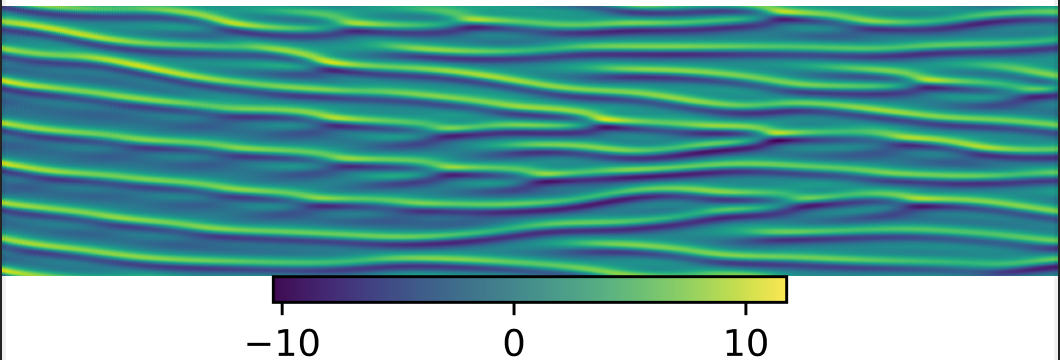
\includegraphics[width=.8\textwidth]{fig/ks.jpg} 
		\label{fig:stats}
	\end{figure}
	\begin{figure}[ht] 
		\centering 
		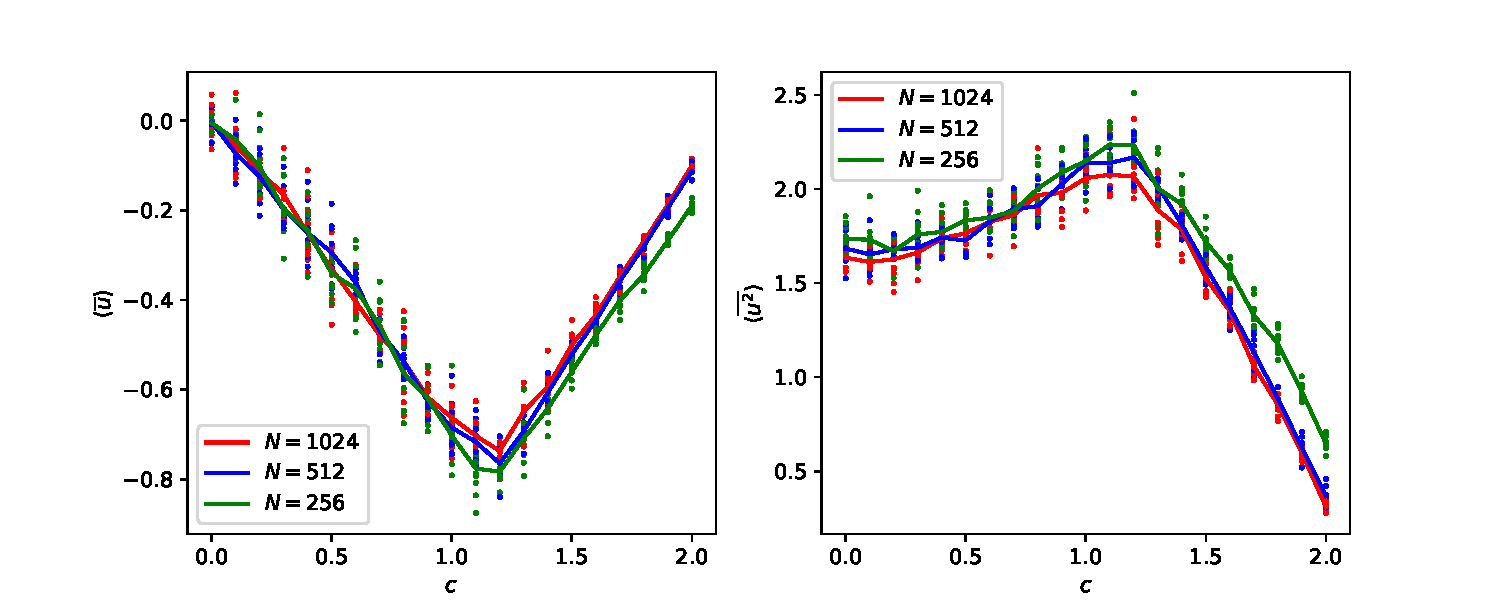
\includegraphics[width=\textwidth]{fig/ks_c_stats.pdf} 
		\label{fig:stats}
	\end{figure}
\end{frame}


\begin{frame}{SGS modeling of the KS equation}
	We use the simulatiosn of KS equation on two grid resolutions (256, 1024).
	Denote a projection operator from the fine grid to the coarse grid as $\opP$
	and numerical scheme as $f_{1024}, f_{256}$, the SGS model we want to handle
	is given by
	\begin{equation}
		\tau_{256} = \opP(f_{1024}(u_{1024})) - f_{256}(\opP u_{1024})
		\sim p(\cdot | u_{256}).
	\end{equation}
\end{frame}


\begin{frame}{Multivalue issue}
	\begin{figure}[ht]
		\centering
		\begin{subfigure}[b]{\textwidth}
			\centering
			
\includegraphics[width=\textwidth]
			{fig/regression_uxx_tau_err_scatter.png}
		\end{subfigure}
		\begin{subfigure}[b]{\textwidth}
			\centering
			
\includegraphics[width=\textwidth]
			{fig/regression_uxxxx_tau_err_scatter.png}
		\end{subfigure}
	\end{figure}
\end{frame}


\begin{frame}{A priori and a posteriori}
	\begin{figure}[ht]
		\centering
		\begin{subfigure}[b]{0.33\textwidth}
			\centering 
			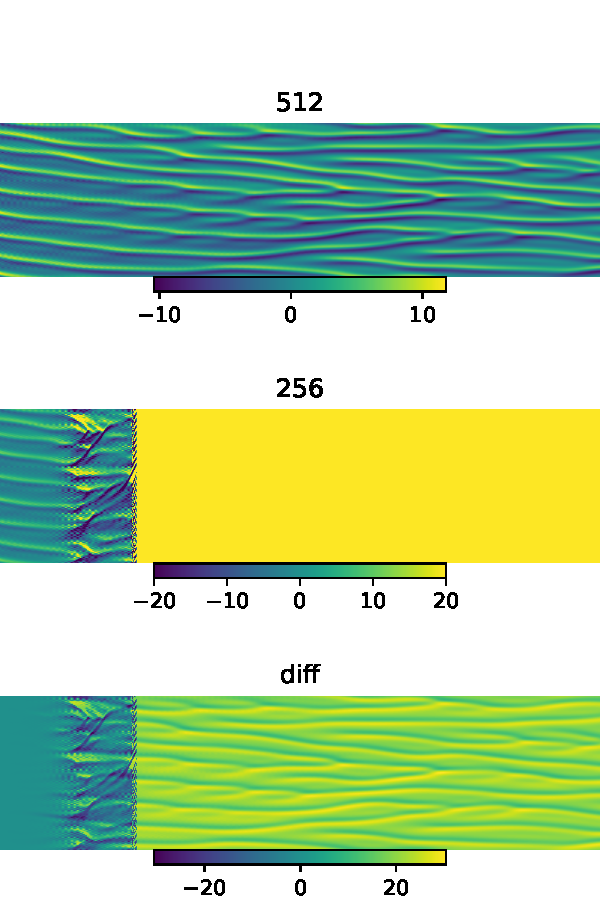
\includegraphics[width=\textwidth]
			{fig/ks_nu0.1_N1512N2256_correct_cmp_lr1e-4.pdf} 
			\caption{validation loss: 3.5000e-05} 
		\end{subfigure}
		\begin{subfigure}[b]{0.33\textwidth}
			\centering 
			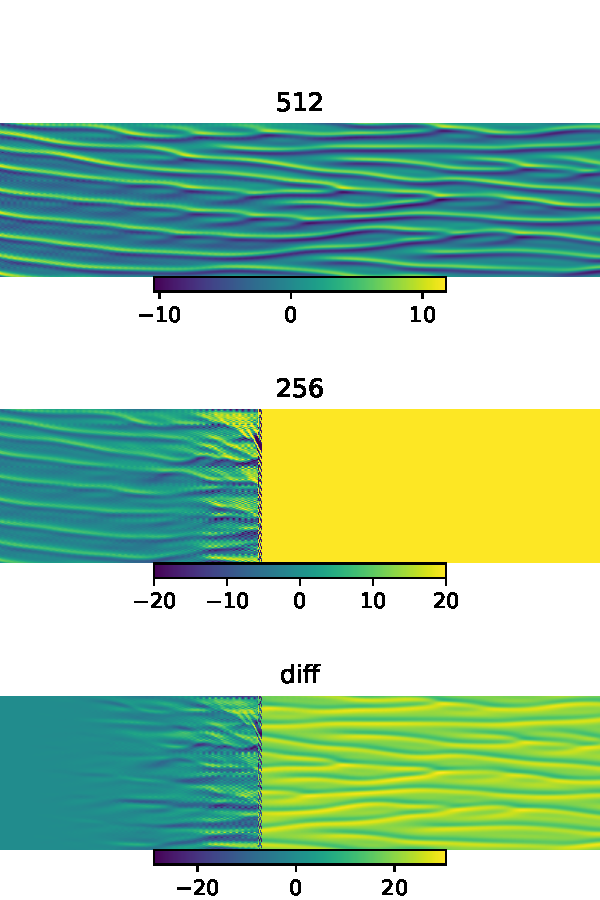
\includegraphics[width=\textwidth]{fig/ks_nu0.1_N1512N2256_correct_cmp_lr2e-4.pdf} 
			\caption{validation loss: 1.3050e-05} 
		\end{subfigure}
		\begin{subfigure}[b]{0.33\textwidth}
			\centering 
			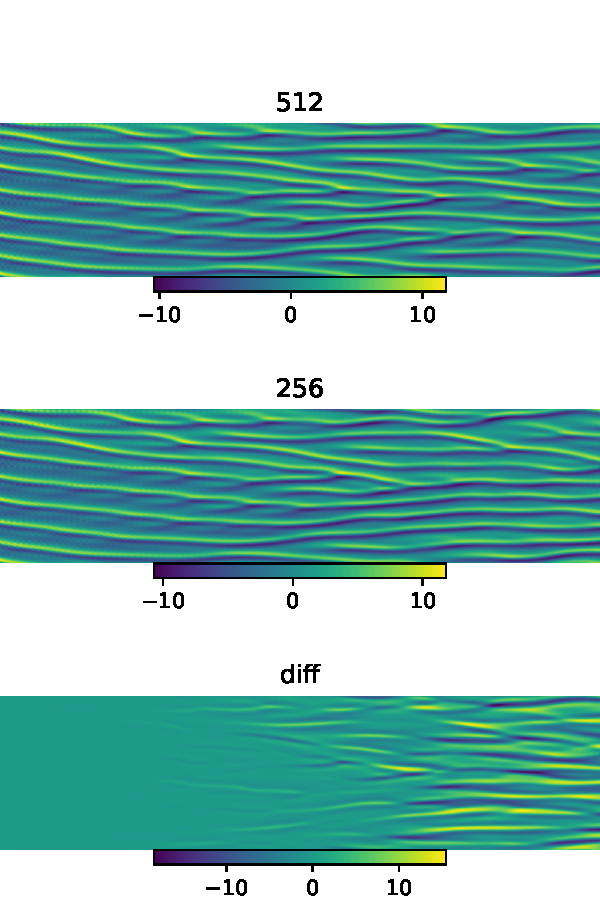
\includegraphics[width=\textwidth]{fig/ks_nu0.1_N1512N2256_correct_cmp_lr5e-4.pdf} 
			\caption{validation loss: 2.8155e-05}  
		\end{subfigure}
	\end{figure}
\end{frame}


\begin{frame}{Proposed model}
	We model the relation between the input features and the SGS stress by
	a conditional probability $p_{\theta}(\tau | \overline{u})$
	Intuitively speaking, this model can not only capture the ``average''
	behavior of the SGS stress but also the {\color{red}uncertainty} of the
	stress depends on how complex the probability family we choose. For
	example, by using Gaussian family, we also capture the variation of the
	stress.

	This methodology is also recognized by the molecular dynamics community,
	e.g. molecular docking.
\end{frame}


\begin{frame}{Optimizing the model}
	Instead of using the MSE as the loss function, we optimize our model by
	maximize the likelihood over data:
	\begin{equation}
		\begin{aligned}
			\min_{\theta} &\sum_{i=1}^{N}\frac{(y_i - \mu_{\theta}(x_i) )^2}
			{2(\sigma_{\theta}(x_i))^2} + \log \sigma_{\theta}(x_i),		\\
			\min_{\theta} &\sum_{i=1}^{N}-\log\lp \sum_{j=1}^M \frac{\text{softmax}
			(c_{\theta}^j(x_i))}{\sigma_{\theta}^j(x_i)}
			\exp\lb-\frac{(y_i - \mu_{\theta}^j(x_i) )^2} 
			{2(\sigma_{\theta}^j(x_i))^2} \rb\rp.
		\end{aligned}
	\end{equation}
	Currently, we naively use the Adam solver to optimize this non-linear
	optimization problem.
\end{frame}


\begin{frame}{Integrating in the simulation}
	How can we deploy this model in the simulation?
	\begin{equation}
		\begin{aligned}
			\text{Gaussian: } u_i & \Longrightarrow \mu_{\theta}(u_i), \sigma_{\theta}(u_i),
			z \sim N(0, 1), \\
			\tau_{ij} & = \mu_{\theta}(u_i) + \sigma_{\theta}(u_i)z,	\\
			\text{Gaussian mixture: } u_i & \Longrightarrow \mu_{\theta}^j(u_i), \sigma_{\theta}^j(u_i),
			z \sim N(0, 1), j \sim [M], \\
			\tau_{i} & = \mu_{\theta}^j(u_i) + \sigma_{\theta}^j(u_i)z,	\\
		\end{aligned}
	\end{equation}
	There is temporal and spatial consistency issue. Should we use the same
	latent variable $z$ for all the grid points at all the time step or we
	should use different $z_i$ for different $u_i$?
\end{frame}


\begin{frame}{Comparison with the regression-based method}
	\begin{equation*}
		\begin{aligned}
			\la\overline{u}\ra &= \frac{1}{LT}\int_{[0, L]}\int_{t}^{t+T} u(x, t)dt dx,
			\\
			\la\overline{u^2}\ra &= \frac{1}{LT}\int_{[0, L]}\int_{t}^{t+T}
			u^2(x, t)dt dx, \\
		\end{aligned}
	\end{equation*}
	\begin{figure}[ht]
		\centering
		\begin{subfigure}[b]{0.48\textwidth}
				\centering
				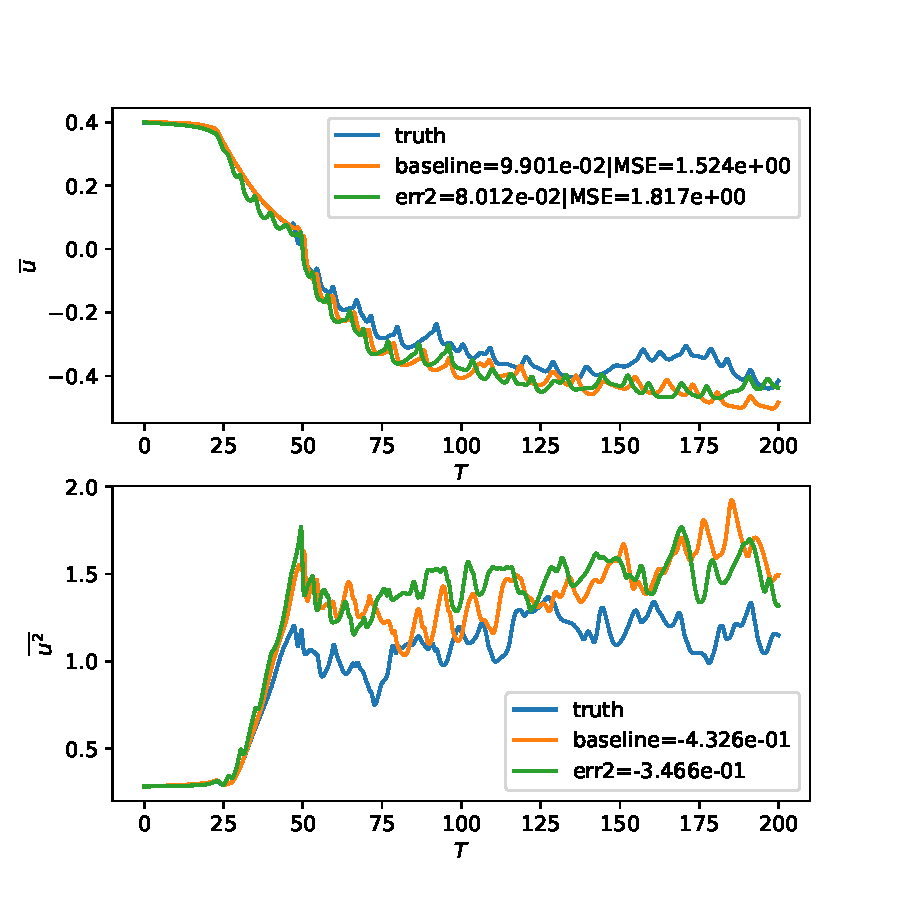
\includegraphics[width=\textwidth]
				{fig/ks_nu1_N1023n10_regression_cmp_stats.pdf}
		\end{subfigure}
		\begin{subfigure}[b]{0.48\textwidth}
				\centering
				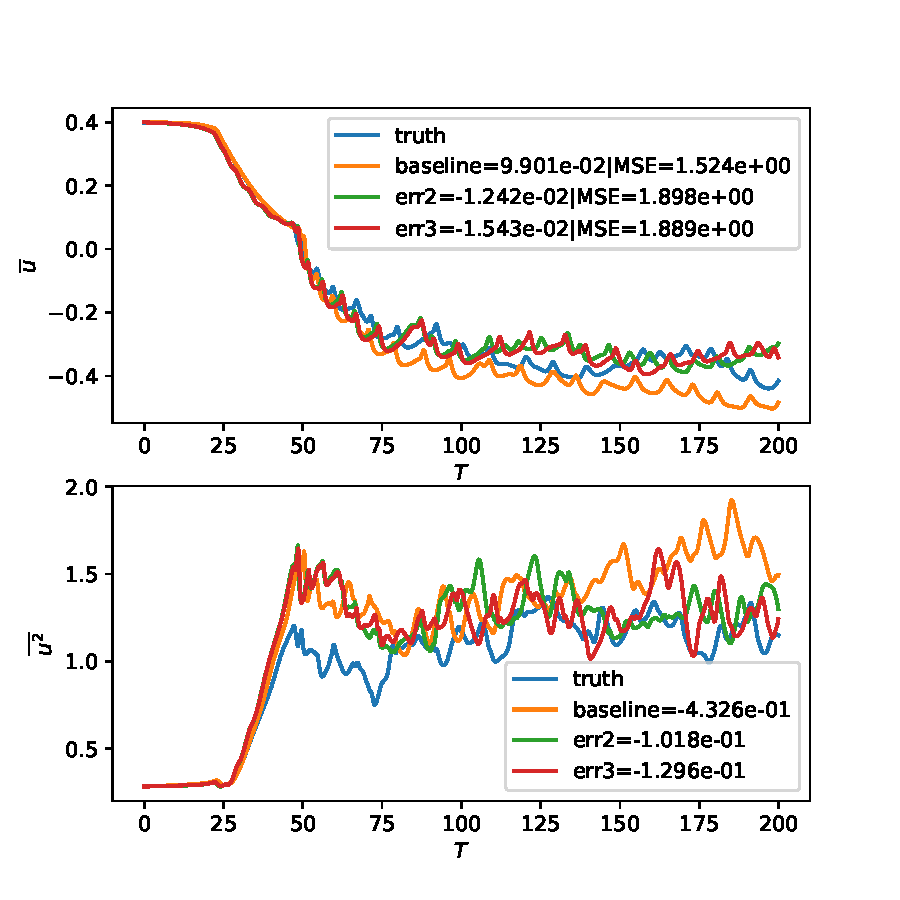
\includegraphics[width=\textwidth]
				{fig/ks_nu1_N1023n10_gaussian_cmp_stats.pdf}
		\end{subfigure}
		\label{fig:cmp_stats1}
	\end{figure}
\end{frame}


\begin{frame}{More experiments}
	\begin{figure}[ht] 
		\centering 
		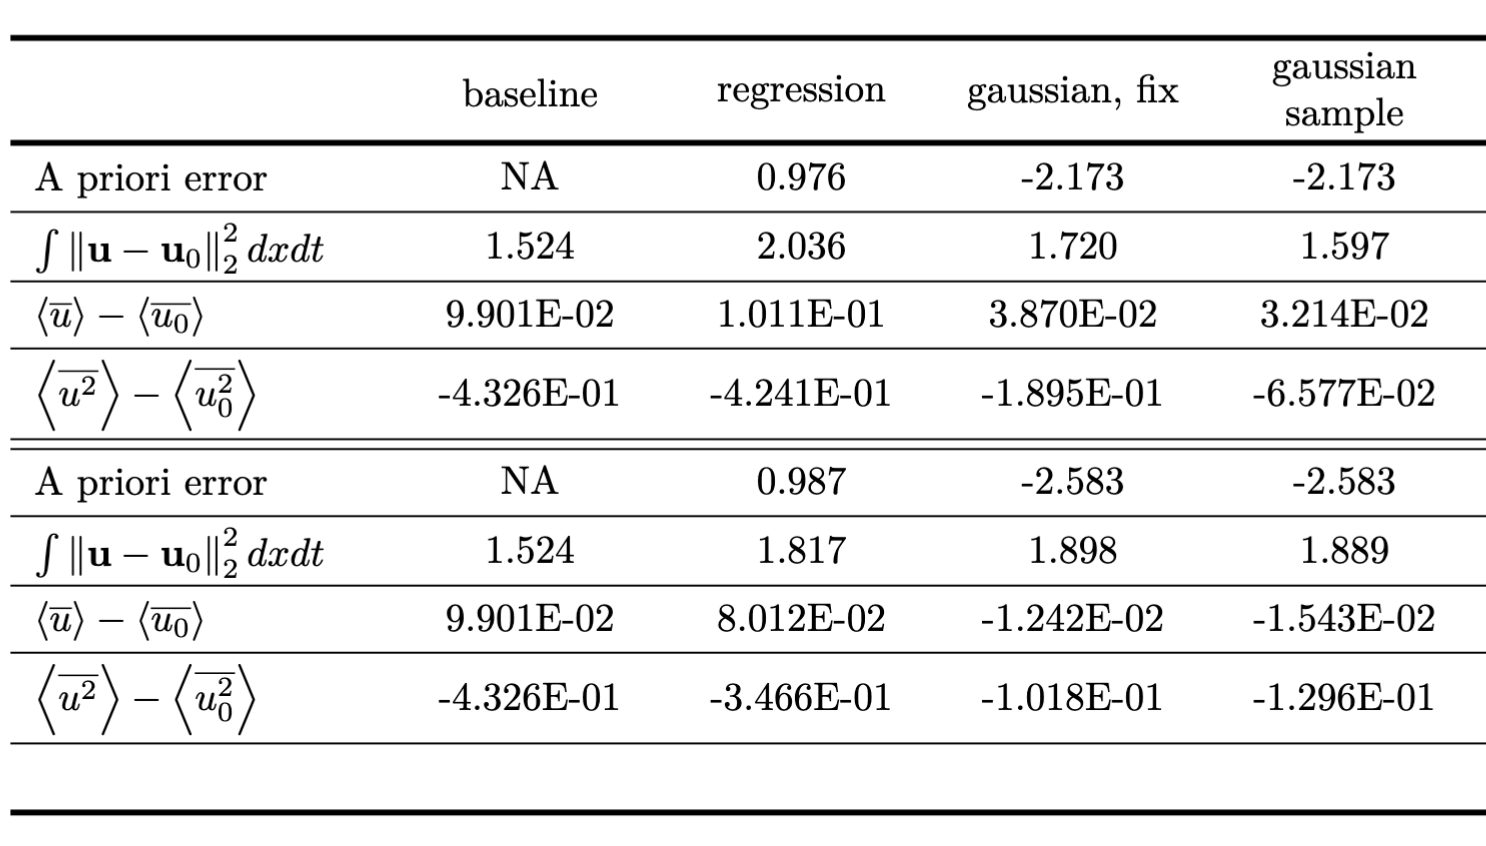
\includegraphics[width=\textwidth]{fig/table.jpg} 
	\end{figure}
\end{frame}


\begin{frame}{Future work}
	\begin{itemize}
		\item 1. Implement more expressive generative models for SGS modeling and
		investigate their performance.
		\item 2. Deploy to practical problems: Subgrid-scale modeling in large
		eddy simulation of the
		urban environment.
		\item 3. Theoretical understanding of the difference between
		regression-based and generative-based SGS modeling, especially in different
		application scenarios such as CFD and MD.
	\end{itemize}
\end{frame}

% \begin{frame} % Use [allowframebreaks] to allow automatic splitting across slides if the content is too long
%     \frametitle{References}
 
%     \begin{thebibliography}{99} % Beamer does not support BibTeX so references must be inserted manually as below, you may need to use multiple columns and/or reduce the font size further if you have many references
%         \footnotesize % Reduce the font size in the bibliography
 
% 		\bibitem[BDI]{bdi}
% 		M. Benjamin, S. Domino, and G. Iaccarino
% 		\newblock Neural Networks for Large Eddy Simulations of Wall-bounded Turbulence: Numerical Experiments and Challenges
% 		\newblock \emph{The European Physical Journal E}

% 		\bibitem[Zhao 2024]{ds}
%         J. Zhao and Q. Li (2024)
%         \newblock Mitigating Distribution Shift in Machine Learning-augmented Hybrid Simulation
%         \newblock \emph{Arxiv preprint https://arxiv.org/pdf/2401.09259}

%         \bibitem[S.A. and Q.L., 2024]{nigbms}
%         S. Arisaka and Q. Li (2024)
%         \newblock Accelerating Legacy Numerical Solvers by Non-intrusive Gradient-based Meta-solving
%         \newblock \emph{International Conference on Machine Learning 2024}
 
        
%     \end{thebibliography}
% \end{frame}

\end{document}